\documentclass[a4paper,14pt]{extarticle}
\usepackage{../../tex-shared/report-layout}

\renewcommand{\mylabnumber}{3}
\renewcommand{\mylabtitle}{Задача дисперсионного анализа. Методы дисперсионного анализа. Однофакторный дисперсионный анализ}
\renewcommand{\mysubject}{Интеллектуальный анализ данных}
\renewcommand{\mylecturer}{Сырых О.А.}

\begin{document}
\begin{titlepage}
    
    \thispagestyle{empty}
    
    \begin{center}
        
        Министерство науки и Высшего образования Российской Федерации \\
        Севастопольский государственный университет \\
        Кафедра ИС
        
        \vfill

        Отчет \\
        по лабораторной работе №\mylabnumber \\
        \enquote{\mylabtitle} \\
        по дисциплине \\
        \enquote{\MakeTextUppercase{\mysubject}}

    \end{center}

    \vspace{1cm}

    \noindent\hspace{7.5cm} Выполнил студент группы ИС/б-17-2-о \\
    \null\hspace{7.5cm} Горбенко К. Н. \\
    \null\hspace{7.5cm} Проверил \\
    \null\hspace{7.5cm} \mylecturer

    \vfill

    \begin{center}
        Севастополь \\
        \the\year{}
    \end{center}

\end{titlepage}

\section{Цель работы}
\begin{itemize}
    \item приобрести практические навыки в проведении дисперсионного анализа по
          экспериментальным данным;
    \item исследовать возможности языка R для проведения дисперсионного анализа.
\end{itemize}

\section{Задание на работу}
\begin{enumerate}
    \item Создать набор данных согласно варианту;
    \item Провести однофакторный дисперсионный анализ в среде \code{Rcmdr}.
    \item По результатам дисперсионного анализа сформулировать выводы.
    \item Построить диаграмму, отображающую средние значения и их доверительные
          интервалы для каждой группы.
\end{enumerate}

Задача: в процессе исследования влияния цены за единицу продукции на объем
продаж (шт.) в месяц были получены следующие результаты:

\begin{table}[H]
    \caption{Данные по варианту}
    \begin{tabular}{ | c | r | r | r | r | }
        \hline
        \multirow{2}{*}{Номер наблюдения} & \multicolumn{4}{c |}{Цена за единицу продукции} \\ \cline{2-5}
        & 1000-1100 & 1100-1200 & 1200-1300 & 1300-1500 \\ \hline
        1 & 215 & 218 & 214 & 211 \\ \hline
        2 & 221 & 214 & 217 & 210 \\ \hline
        3 & 222 & 220 & 210 & 208 \\ \hline
        4 & 219 & 221 & & 209 \\ \hline
        5 & & 213 & & \\ \hline
    \end{tabular}
\end{table}

\section{Дисперсионный анализ данных по варианту}
\subsection{Создание набора данных}
Создадим .csv файл следующего содержания:

\begin{lstlisting}
num,sales1000-1100,sales1100-1200,sales1200-1300,sales1300-1500
1,215,218,214,211
2,221,214,217,210
3,222,220,210,208
4,219,221,,209
5,,213,,
\end{lstlisting}

\subsection{Дисперсионный анализ в MS Excel}
Откроем полученный .csv файл в MS Excel, с помощью пакета \enquote{Пакет
анализа} проведем однофакторный дисперсионный анализ данных. Результат анализа
приведен на рисунке \ref{fig:sales-data-excel}.

\begin{figure}[H]
    \centering
    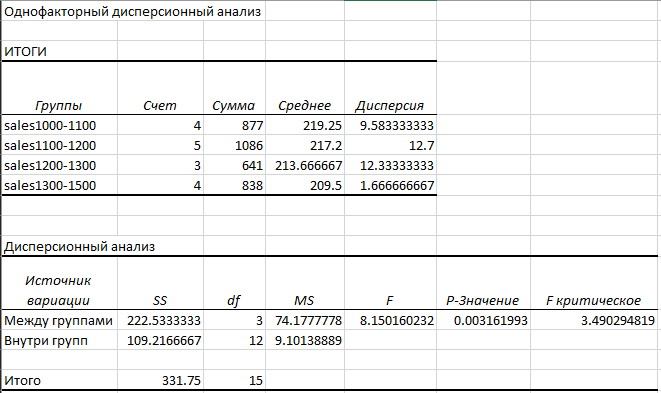
\includegraphics[width=.8\linewidth]{sales-data-excel}
    \caption{Результат дисперсионного анализа в Excel}
    \label{fig:sales-data-excel}
\end{figure}

По среднему значению количества продаж в зависимости от цены товаров отличаются
незначительно: лучший результат при цене 1000-1100, худший - при цене 1300-1500.
При этом сохраняется тенденция к уменьшению количества продаж при увеличении
цены.

Для цены 1300-1500 количества продаж по дням практически не отличаются (208,
209, 210, 211), соответственно дисперсия принимает малые значения.

Т.к $F > F _\textup{крит}$, значит отвергнута нулевая гипотеза и принята первая
гипотеза с вероятностью ошибки $\alpha = 0,05$ можно утверждать, что влияние
фактора (цены) на результирующий признак (количество продаж) существенно.

\subsection{Дисперсионный анализ средствами языка R}
Выполним дисперсионный анализ данных по варианту с помощью средств языка R.
Результат изображен на рисунке \ref{fig:sales-data-R}.

\begin{figure}[H]
    \centering
    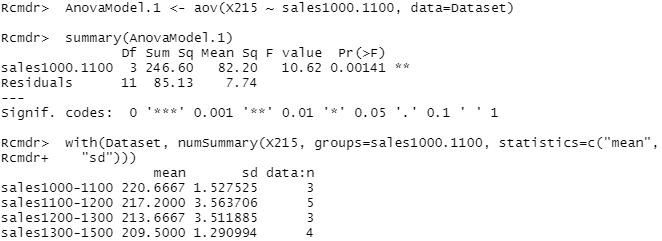
\includegraphics[width=.8\linewidth]{sales-data-R}
    \caption{Результат дисперсионного анализа средствами языка R}
    \label{fig:sales-data-R}
\end{figure}

Диаграмма средних значений и их доверительных интервалов изображена на рисунке
\ref{fig:sales-data-plot-of-means}.

\begin{figure}[H]
    \centering
    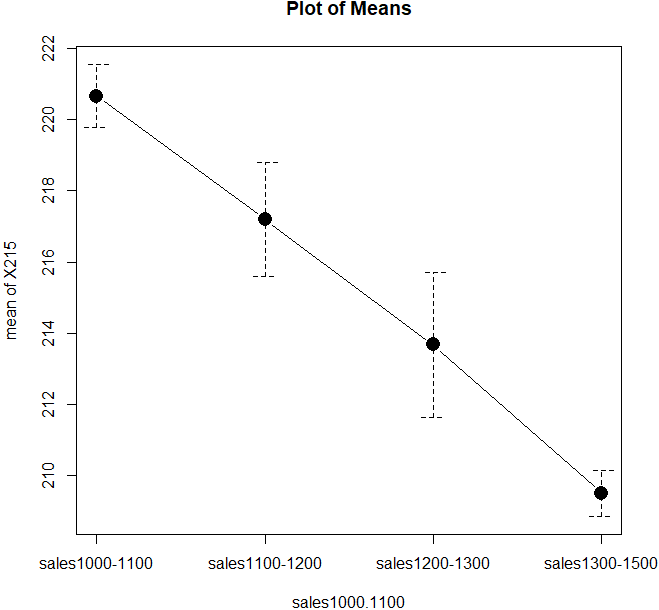
\includegraphics[width=.5\linewidth]{sales-data-plot-of-means}
    \caption{Диаграмма средних значений и их доверительных интревалов для данных по варианту}
    \label{fig:sales-data-plot-of-means}
\end{figure}

Сравнение средних значений показало, что количество продаж наивысшее у товаров с
ценой 1000-1100, наинизшее у товаров 1300-1500. Т.к. $Pr(>F)$ составляет 0.14\%,
мы отвергаем нулевую гипотезу. Значение F-критерия составило 10.62.

\section{Дисперсионный анализ своих экспериментальных данных в MS Excel}
\subsection{Создание набора данных}
Для анализа выберем зависимость количества заражений от индекса строгости.
Преобразуем экспериментальные данные к следующему виду:

\begin{figure}[H]
    \centering
    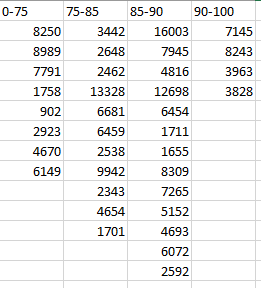
\includegraphics[width=.3\linewidth]{total-cases-stringency-converted}
    \caption{Преобразованные данные}
    \label{fig:total-cases-stringency-converted}
\end{figure}

\subsection{Дисперсионный анализ в Excel}
Выполним дисперсионный анализ в MS Excel. Результат выполнения представлен на
рисунке \ref{fig:my-data-excel}.

\begin{figure}[H]
    \centering
    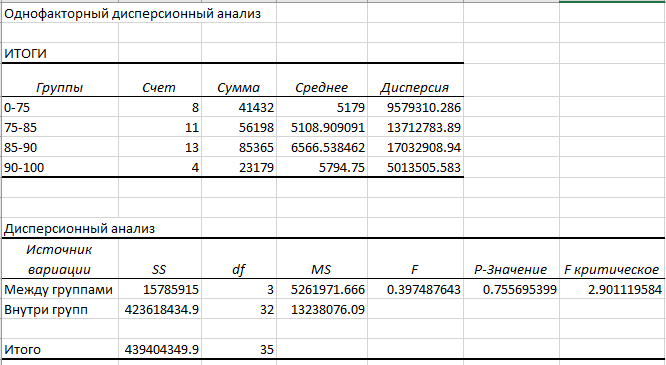
\includegraphics[width=.8\linewidth]{my-data-excel}
    \caption{Результат дисперсионного анализа в MS Excel}
    \label{fig:my-data-excel}
\end{figure}

Для интервала индекса строгости 85-90 наблюдается наибольшее среднее значение
количества заражений. При этом не наблюдается тенденции к уменьшению количества
заражений при увеличении индекса строгости. $F < F _\textup{крит}$, нулевую
гипотезу отвергнуть нельзя, связь между переменными не доказана.

\subsection{Дисперсионный анализ средствами языка R}
Выполним дисперсионный анализ данных по варианту с помощью средств языка R.
Результат изображен на рисунке \ref{fig:my-data-R}.

\begin{figure}[H]
    \centering
    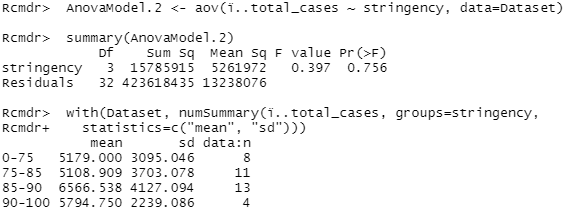
\includegraphics[width=.8\linewidth]{my-data-R}
    \caption{Результат дисперсионного анализа средствами языка R}
    \label{fig:my-data-R}
\end{figure}

Диаграмма средних значений и их доверительных интервалов для своих данных
приведена на рисунке \ref{fig:my-data-plot-of-means}.

\begin{figure}[H]
    \centering
    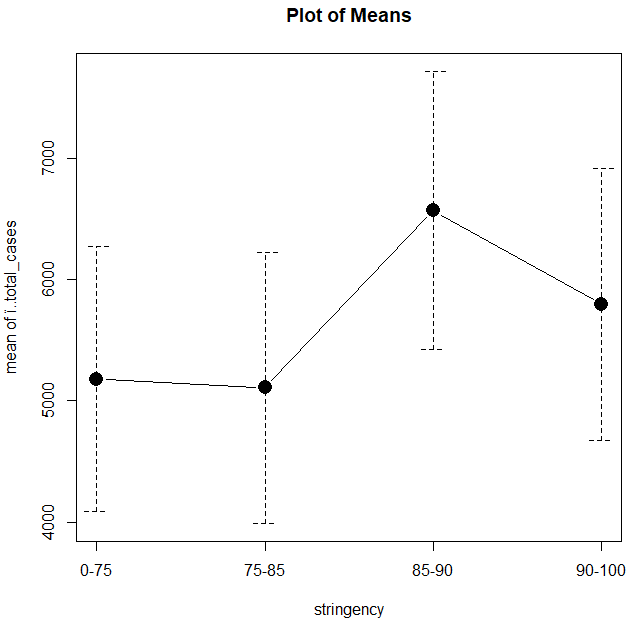
\includegraphics[width=.5\linewidth]{my-data-plot-of-means}
    \caption{Диаграмма средних значений и их доверительных интервалов для своих данных}
    \label{fig:my-data-plot-of-means}
\end{figure}

Значение отношения межгрупповой изменчивости к внутригрупповой равно 0.397, то
есть мы отклонились от левой части распределения Фишера. Уровень значимости
говорит о том, что получить такое распределение мы можем с вероятностью 75\%.
Значит, влияние рассматриваемого фактора на результативный признак несущественно.

\section*{Выводы}
В ходе выполнения лабораторной работы были приобретены практические навыки в
проведении дисперсионного анализа по экспериментальным данным. Также был получен
опыт анализа данных с помощью однофакторного дисперсионного анализа.

\end{document}